\documentclass[12pt]{article}
\usepackage{times}
\usepackage[english]{babel}
\usepackage[utf8x]{inputenc}
\usepackage[colorinlistoftodos]{todonotes}
\usepackage[margin=1in]{geometry}
\usepackage{graphicx}
\usepackage{epstopdf}
\usepackage{cite}
\usepackage{listings}
\usepackage{dtklogos}
\usepackage{wrapfig}
\usepackage{subfigure}
\usepackage{amsmath}
\usepackage{amsthm}
\usepackage{amssymb}
\usepackage{amscd}
\usepackage{caption}
\usepackage{etoolbox}
\usepackage{fancyhdr}
\usepackage{stackengine}
\usepackage[export]{adjustbox}
\patchcmd{\thebibliography}{\section*{\refname}}{}{}{}
\usepackage[document]{ragged2e}    %This causes text to left align
\usepackage[colorlinks=true, linkcolor=black,citecolor=black,urlcolor=blue]{hyperref}
\bibliographystyle{IEEEtran}
\DeclareGraphicsRule{.tif}{png}{.png}{`convert #1 `dirname #1`/`basename #1 .tif`.png}

\title{MCHE 474: Lab 5}

\begin{document}
\lefthyphenmin3
\righthyphenmin4
% \pretolerance=2000
% \tolerance=500 
% \emergencystretch=10pt
%\raggedright     %Stops LaTeX from automatically hyphenating the right margin to fit better
%Combine this with \usepackage[document]{ragged2e} to get a text align left similar to natural MS Word


%-------------------------------------------------------------
%Start of Paper
%-------------------------------------------------------------

%%%%%%%%%%%%%%%%%%%%%%%%%%%%%%%%%%%%%%%%%%%%%%%%%%%%%%
%%%%%%%%%%%%%%%%%%%%%%% TITLE PAGE %%%%%%%%%%%%%%%%%%%%%%%%
%%%%%%%%%%%%%%%%%%%%%%%%%%%%%%%%%%%%%%%%%%%%%%%%%%%%%%

\begin{titlepage}

\newcommand{\HRule}{\rule{\linewidth}{0.5mm}} % Defines a new command for the horizontal lines, change thickness here

\center % Center everything on the page
 
%----------------------------------------------------------------------------------------
%	Heading Section
%----------------------------------------------------------------------------------------

\textsc{\LARGE University of Louisiana at Lafayette}\\[1.5cm] % Name of your university/college
\textsc{\Large Control Systems}\\[0.5cm] % Major heading such as course name
\textsc{\large MCHE 474}\\[0.5cm] % Minor heading such as course title

%----------------------------------------------------------------------------------------
%	Title Section
%----------------------------------------------------------------------------------------

\HRule \\[0.4cm]
{ \huge \bfseries Lab 5}\\[0.4cm] % Title of your document
\HRule \\[1.5cm]
 
%----------------------------------------------------------------------------------------
%	Author Section
%----------------------------------------------------------------------------------------

\begin{minipage}{0.4\textwidth}
\begin{flushleft} \large
\emph{Author:}\\
\textsc{Matthew J. Begneaud} \\% Your name
\end{flushleft}
\end{minipage}
~
\begin{minipage}{0.4\textwidth}
\begin{flushright} \large
\emph{Professor:} \\
\textsc{Dr. Mostafa A. Elsayed} % Supervisor's Name
\end{flushright}
\end{minipage}\\[1.5cm]

% If you don't want a supervisor, uncomment the two lines below and remove the section above
%\Large \emph{Author:}\\
%John \textsc{Smith}\\[3cm] % Your name

%----------------------------------------------------------------------------------------
%	Date Section
%----------------------------------------------------------------------------------------

{\textsc{\large \today}}\\[2cm] % Date, change the \today to a set date if you want to be precise

%----------------------------------------------------------------------------------------
%	Logo Section
%----------------------------------------------------------------------------------------


\includegraphics[width=5in]{UL_logo.jpg}\\[1cm] % Include a department/university logo - this will require the graphicx package
 
%----------------------------------------------------------------------------------------

\vfill % Fill the rest of the page with whitespace

\end{titlepage}

%%%%%%%%%%%%%%%%%%%%%%%%%%%%%%%%%%%%%%%%%%%%%%%%%%%%%%
%%%%%%%%%%%%%%%%%%%%%%% TABLE OF CONTENTS %%%%%%%%%%%%%%%%%%%
%%%%%%%%%%%%%%%%%%%%%%%%%%%%%%%%%%%%%%%%%%%%%%%%%%%%%%

\tableofcontents

\listoffigures

\listoftables

\section*{\fontsize{12}{12}\selectfont \large List of Symbols}
\addcontentsline{toc}{section}{List of Symbols} % Add for each section
$G$ = Plant Function \\
$G_{c}$ = PID Controller \\
$s$ = Laplace Domain Variable \\
$PID$ = Proportional-Integral-Derivative Controller \\
$K$ = Gain \\
$K_{P}$ = Proportional Gain \\
$K_{I}$ = Integral Gain \\
$K_{D}$ = Derivative Gain \\

\newpage

%%%%%%%%%%%%%%%%%%%%%%%%%%%%%%%%%%%%%%%%%%%%%%%%%%%%%%
%%%%%%%%%%%%%%%%%%%%%%% REPORT %%%%%%%%%%%%%%%%%%%%%%%%%%
%%%%%%%%%%%%%%%%%%%%%%%%%%%%%%%%%%%%%%%%%%%%%%%%%%%%%%


\section*{\fontsize{12}{12}\selectfont \large Introduction}
\addcontentsline{toc}{section}{Introduction} % Add for each section
This lab was conducted using MATLAB to analyze a control system. The system's plant is given in Equation 1. The system root-locus is plotted and used for analysis. A PID controller is then implemented into the system in order to improve the system's performance. The gains for the PID controller are chosen based on the zeros found in the root-locus analysis.
\bigskip

\begin{equation}
G = \frac{1}{(s+2)(s+3)}
\end{equation}
\bigskip

\begin{equation}
G_{c} = \frac{K_{d}(s+Z_{1})(s+Z_{2})}{s}
\end{equation}
\bigskip


\section*{\fontsize{12}{12}\selectfont \large Theory}
\addcontentsline{toc}{section}{Theory} % Add for each section
The root-locus plot of a system can reveal much about the behavior of the system. The root-locus is a plot showing the location of zeros and poles of the system. Zeros of a system are the values of $s$ that cause the numerator of the transfer function to equal zero. Poles are the values of $s$ that cause the denominator of the transfer function to equal zero. The zeros and poles of a system are often times complex numbers. For this reason, the root-locus plot of a system is plotted on the real-imaginary plane. The root-locus plot shows how the poles and zeros change as an applied gain $K$ goes from $0$ to $\infty$.
\bigskip

A PID is a feedback controller which accounts for not just one state of error, but three, in order to modify the input to the system to achieve the desired state. The equation for a PID controller is shown in Equation 3, and is rewritten in Equation 4.
\bigskip

\begin{equation}
PID= K_{P} + \frac{K_{I}}{s} + K_{D}s
\end{equation}

\begin{equation}
PID= \frac{K_{D}s^2 + K_{P}s + K_{I}}{S}
\end{equation}
\bigskip

The effect of the proportional, integral, and derivative components of the controller are weighted by their gains KP, KI, and KD respectively. Adjusting these gains allows for the PID con- troller to be tailored to fit the system and the desired performance. Adjusting the proportional
gain changes how intensely the controller reacts to error. Adjusting the integral gain changes
how quickly accumulated error is accounted for by increasing the controller output. Adjusting the derivative gain changes how quickly the controller reacts to a change in the rate of error change, which is useful for situations where the error changes signs frequently (like an autonomous vehicle which needs to stick to a straight course).
\bigskip


\section*{\fontsize{12}{12}\selectfont \large Procedure \& Analysis}
\addcontentsline{toc}{section}{Procedure \& Analysis} % Add for each section
The root-locus of the system without the compensation of PID control is shown in Figure 1. The step response of the system is plotted in Figure 2 and the system performance criteria are shown in Figure 3. The uncompensated system can be thought of as having a gain $K = 1$.
\bigskip

% Figrues 1-3
\begin{figure}[h!] %  figure placement: here, top, bottom, or page
   \centering
   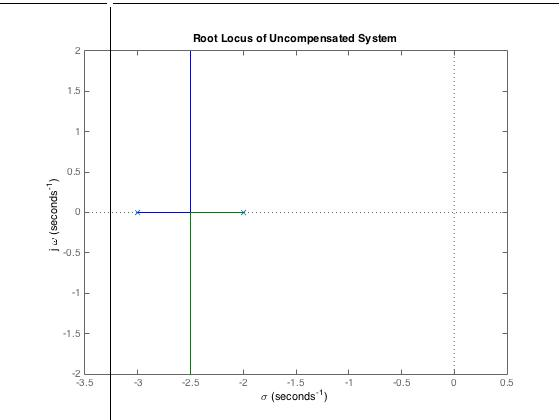
\includegraphics[width=4.5in]{uncompensated_root_locus.jpg} 
   \caption{Uncompensated System Root-Locus}
   \label{fig:example}
\end{figure}

\begin{figure}[h!] %  figure placement: here, top, bottom, or page
   \centering
   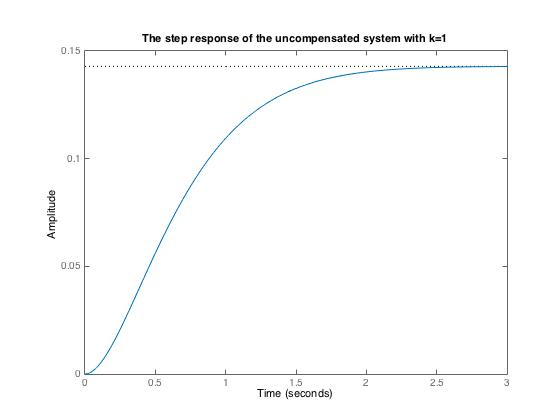
\includegraphics[width=5in,height=3in]{uncompensated_sys_time_resp.jpg} 
   \caption{Uncompensated System Step Response ($K=1$)}
   \label{fig:example}
\end{figure}

\newpage

\begin{figure}[h!] %  figure placement: here, top, bottom, or page
   \centering
   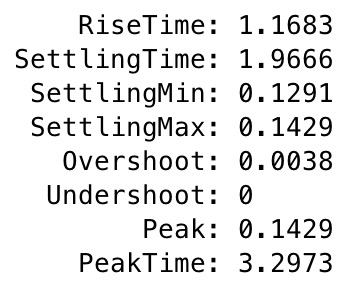
\includegraphics[width=2in,height=1.5in]{uncompensated_sys_step_info.jpg} 
   \caption{Uncompensated System Step Response Performance ($K=1$)}
   \label{fig:example}
\end{figure}

\bigskip

 The PID controller was then introduced to the system, where $Z_{1,2} = -3 \pm j$. The root-locus of the compensated system is shown in Figure 4. The highest point on the root-locus plot was then chosen to define a value of $K_{d}$ and the system step response was plotted for this gain in Figure 5. The performance criteria for the system with this $K_{d}$ is shown in Figure 6.
\bigskip
 
The gain $K_{d}$ was then chosen so that the system has even less damping. The system step response with this gain is plotted in Figure 7 and the performance criteria are shown in Figure 8. The performance criteria of all three step system configurations is tabulated in Table 1. 
\bigskip

% Figures 4-8
\begin{figure}[h!] %  figure placement: here, top, bottom, or page
   \centering
   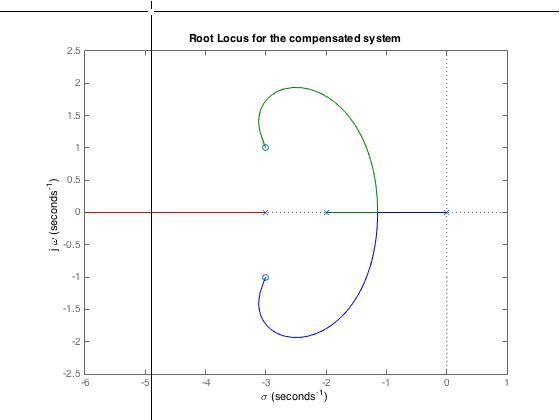
\includegraphics[width=5in]{compensated_root_locus.jpg} 
   \caption{Compensated System Root-Locus}
   \label{fig:example}
\end{figure}

\newpage

\begin{figure}[h!] %  figure placement: here, top, bottom, or page
   \centering
   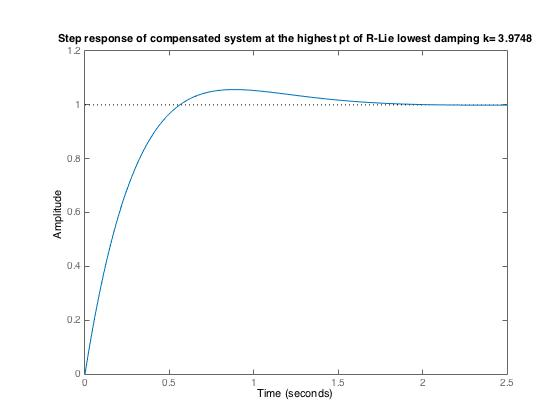
\includegraphics[width=5.5in,height=4in]{compensated_sys_highest_rl_time_resp.jpg} 
   \caption{Compensated System Step Response ($K=3.9748$)}
   \label{fig:example}
\end{figure}

\bigskip
\bigskip
\bigskip

\begin{figure}[h!] %  figure placement: here, top, bottom, or page
   \centering
   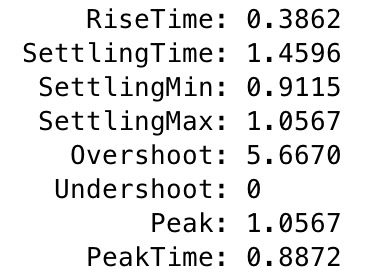
\includegraphics[width=2in,height=1.5in]{compensated_sys_highest_rl_step_info.jpg} 
   \caption{Compensated System Step Response Performance ($K=3.9748$)}
   \label{fig:example}
\end{figure}

\newpage

\begin{figure}[h!] %  figure placement: here, top, bottom, or page
   \centering
   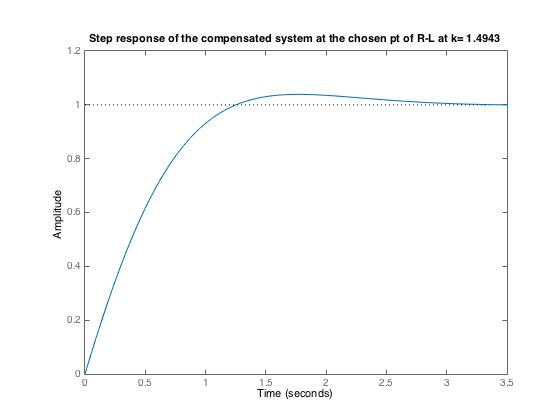
\includegraphics[width=5.5in,height=4in]{compensated_sys_chosen_rl_time_resp.jpg} 
   \caption{Compensated System Step Response ($K=1.4943$)}
   \label{fig:example}
\end{figure}

\bigskip
\bigskip
\bigskip

\begin{figure}[h!] %  figure placement: here, top, bottom, or page
   \centering
   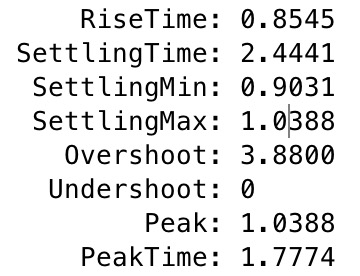
\includegraphics[width=2in,height=1.5in]{compensated_sys_chosen_rl_step_info.jpg} 
   \caption{Compensated System Step Response Performance ($K=1.4943$)}
   \label{fig:example}
\end{figure}

\newpage

% Table 1
\begin{table}[]
\centering
\caption{Comparison of Performance Criteria}
\label{my-label}
\begin{tabular}{cccc}
\hline
\textbf{\begin{tabular}[c]{@{}c@{}}Performance\\ Criteria\end{tabular}} & \textbf{\begin{tabular}[c]{@{}c@{}}Uncompensated System\end{tabular}} & \textbf{\begin{tabular}[c]{@{}c@{}}Compensated System \\ (K=3.9748)\end{tabular}} & \textbf{\begin{tabular}[c]{@{}c@{}}Compensated System \\(K=1.4943)\end{tabular}} \\ \hline
Rise Time (s)                                                           & 1.1683                                                                  & 0.3862                                                                           & 0.8545                                                                           \\
Settling Time (s)                                                       & 1.9666                                                                  & 1.4596                                                                           & 2.4441                                                                           \\
Overshoot (Amplitude)                                                   & 0.0038                                                                  & 5.6670                                                                           & 3.8800                                                                          
\\ \hline

\end{tabular}
\end{table}

\section*{\fontsize{12}{12}\selectfont \large Conclusion}
\addcontentsline{toc}{section}{Conclusion} % Add for each section
The exercises conducted in this lab reinforce the theory learned in the classroom. It is shown that the root-locus plot of a system can show much information about the system. It is also shown that the performance of a system can be improved using a PID controller, which is a tunable feedback controller that accounts for present, past, and future error states of the system. Choosing the zeros of the PID controller to be similar to the zeros of the system plant results in performance improvement for the system. These system characteristics are important for control systems with feedback loops which utilize PID control. With the information obtained from the root-locus, the zeros and gains of the PID controller can be wisely chosen.



%\section*{\fontsize{12}{12}\selectfont \large References}

\begin{thebibliography}{2}

% Example
%\bibitem{Wagner}
%Ng, K., Wagner, S.W., Camelio, J., Emblom, W.J. (2010). ?Experimental Analysis of Micro Tube
%Hydroforming Process.? Transactions of NAMRC of SME, 38, 577-584.

\end{thebibliography}



%\section*{\fontsize{12}{12}\selectfont APPENDIX}

%\begin{table}[h!]
%  \caption{}
%  \includegraphics[width=\linewidth]{table1.png}
%\end{table}




\end{document}







----------------------------Templates-------------------------------

-------------------------Figure-----------------------

\begin{figure}[h!]  
  \centering
    \includegraphics[width=\linewidth]{**file**}
    \caption{Docking Station}
\end{figure}

---------------------------Table-----------------------
\begin{table}[ht]
\caption{Nonlinear Model Results} % title of Table
\centering % used for centering table
\begin{tabular}{c c c c} % centered columns (4 columns)
\hline\hline %inserts double horizontal lines
Case & Method\#1 & Method\#2 & Method\#3 \\ [0.5ex] % inserts table
%heading
\hline % inserts single horizontal line
1 & 50 & 837 & 970 \\ % inserting body of the table
2 & 47 & 877 & 230 \\
3 & 31 & 25 & 415 \\
4 & 35 & 144 & 2356 \\
5 & 45 & 300 & 556 \\ [1ex] % [1ex] adds vertical space
\hline %inserts single line
\end{tabular}
\label{table:nonlin} % is used to refer this table in the text
\end{table}



probably best to insert as an image from excel

\bigskip\\
\begin{table}[h!]
  \caption{}
  \includegraphics[width=\linewidth]{**file**}
\end{table}
\bigskip\\





-----------------------------Equations------------------------
-----------------------------Regular
\begin{equation}
a = b + c
\end{equation}

--------------------------------- Multiline
\begin{multline}
a = b + c + d + e + f
+ g + h + i + j \\
+ k + l + m + n + o
\end{multline}

-------------------------------Citations-------------------------
\bibitem{Author last name}
  Last, First., year of publication,
  article name, book(etc) name, from \\
  link goes here

----------------------------------other-----------------------------

equations:
http://moser-isi.ethz.ch/docs/typeset_equations.pdf

citations:
http://library.missouri.edu/engineering/about/guides/asme
https://www.asme.org/shop/proceedings/conference-publications/references